\chapter[Experiment]{Experiment Evaluation}
\label{exp}

	\section{Introduction}
	\label{exp:intro}

		As a way to get the widest possible range of data from the scenes created, two different experiments were planned (\enquote{Experiment 1} and \enquote{Experiment 2}).
		The experiments were set up in a way that a participant in an experiment would either be shown the standard or non-Euclidean game scene first, and once they had successfully navigated around it, they would then be shown the other.
		\enquote{Experiment 1} had the participants viewing the standard scene first and the non-Euclidean scene second, with \enquote{Experiment 2} having the participants view the non-Euclidean scene first and the standard scene second.

		A total of 10 participants from Computer Games Programming and Design courses took part in the experiments, with 5 participants taking part in \enquote{Experiment 1}, and the other 5 \enquote{Experiment 2}.
		Having the participants view the two scenes in different orders allowed for the results of the experiments to not only cover the effects of the respective scenes geometry, but also to see if being exposed to the other environment in any way impacts their immersion to the one they are currently in. % TODO: Reword this?
		$60\%$ of the participants in \enquote{Experiment 1} had used a VR system prior to the experiment, compared to $80\%$ of the participants in \enquote{Experiment 2}.

		During the experiments, participants were asked to fill out a 2 page questionnaire, an unfilled version of which can be seen on page \pageref{appendix:question}.
		After viewing the first scene, participants were asked to fill out the first page of the questionnaire. Once they'd filled the page, they would view the second scene, after which they were asked to fill out the second page. % TODO: Reword this?
		All participants were naive to the purpose of the experiments.

		An Oculus Rift Developer Kit 2 was used as the display device for the experiments, using the included IR camera for six degrees of freedom head tracking within the scenes.
		The same desktop computer was used for all experiments (CPU: Intel Core i7 4790, GPU: NVIDIA GTX 970, RAM: 16GB), to ensure consistent render speeds for each participant.

		The analysis of the gathered results will be covered in three sections. The first will cover the results from all 10 participants solely on the data gathered for the standard scene; The second covers the results from all 10 participants solely on the data from the non-Euclidean scene; Finally, the third covers the comparison between results for the two scene types depending on the experiment. % TODO: Reword this?

	\section{Experiments}
	\label{exp:exp}

		\subsection{Standard Euclidean Geometry}
		\label{exp:exp:standard}

			Having an experiment scene using standard Euclidean geometry which follows a similar layout to the non-Euclidean scene sets a good foundation for the validation of the results. % TODO: Reword this?
			The questionnaire the participants were asked to fill in focused on two main metrics, their personal sense of immersion within the scene, as well as their sense of comfort navigating within the scene.

			\subsubsection{Immersion}

				To judge a participants sense of immersion within the scene, they were asked to rate their sense of immersion on a scale of 1 - 10, with 1 being \enquote{No Immersion} and 10 being \enquote{Fully Immersed}.

				From the gathered results (\autoref{exp:fig:standard_immersion}), the mean rating for immersion in the standard scene was $7$, with a standard deviation of $1$.
				The low standard deviation in the results, coupled with the high mean value shows that a virtual environment which is similar geometrically to the real world has a consistently immersive impact on participants.

				\begin{figure}[h]
					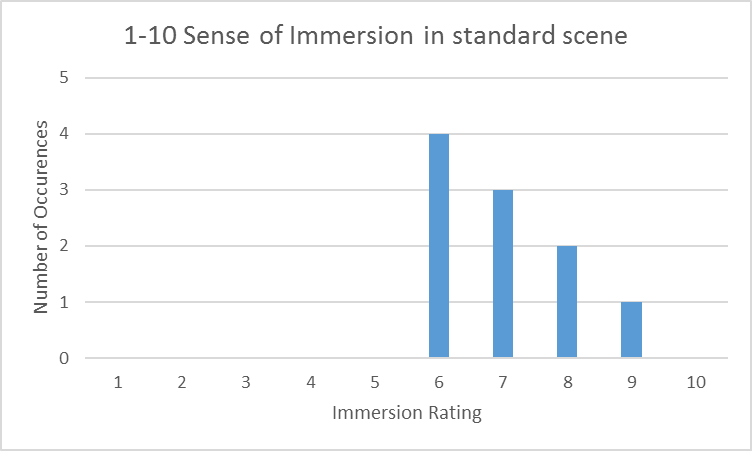
\includegraphics[width=1\textwidth]{Images/Standard_Immersion}
					\centering
					\caption{Immersion rating in standard geometry test scene}
					\label{exp:fig:standard_immersion}
				\end{figure}

				As well as the number rating for immersion, participants were optionally asked to mention what factors positively and negatively influenced their immersion within the scene.
				$40\%$ of the participants commented saying the tracking of their heads in the game scene positively effected their immersion in the scene.
				A further $30\%$ of participants mentioned the scaling and lighting of the scene positively impacted their sense of immersion.

				$40\%$ of participants also mentioned that the method of input for movement within the scene negatively impacted their sense of immersion.

			\subsubsection{Navigation Comfort}

				As with the Immersion questions, participants were asked to rate their sense of comfort navigating the scene on a scale of 1 - 10, with 1 being \enquote{No Comfort}, and 10 being \enquote{Fully Natural}.

				The gathered results (\autoref{exp:fig:standard_comfort}) show a mean value for navigation comfort at $7$, with a standard deviation of $2$.
				Although there is a high mean value for the results, the high standard deviation shows that the navigation comfort within the scene was not consistent between all participants in the scene.

				\begin{figure}[h]
					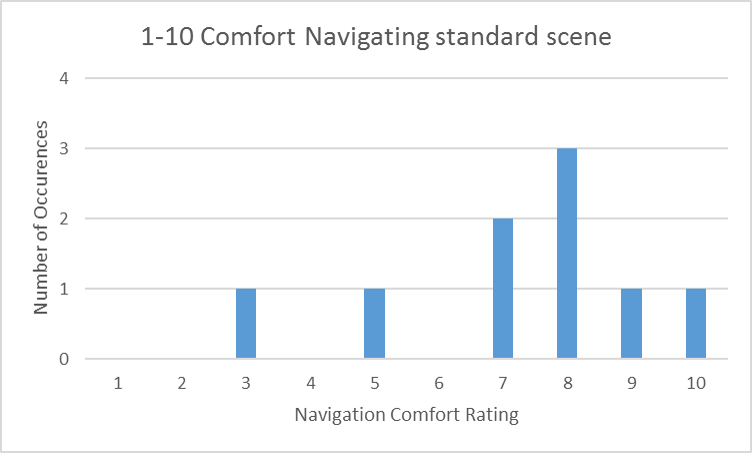
\includegraphics[width=1\textwidth]{Images/Standard_Comfort}
					\centering
					\caption{Navigation Comfort rating in standard geometry test scene}
					\label{exp:fig:standard_comfort}
				\end{figure}

			\subsubsection{Correlation}

				By mapping the results a participant gave in this scene for both metrics on a scatter graph (\autoref{exp:fig:standard_relation}), it is possible to work out whether a users sense of comfort navigating in the scene effects their sense of immersion within it.

				Even though there is a high standard deviation with the results gathered for navigation comfort compared to immersion, there does still appear to be a noticeable positive correlation between the two.
				For this scene, the trend line for immersion and navigation comfort fits on the line of $y = 0.7x + 2.1$.

				\begin{figure}[h]
					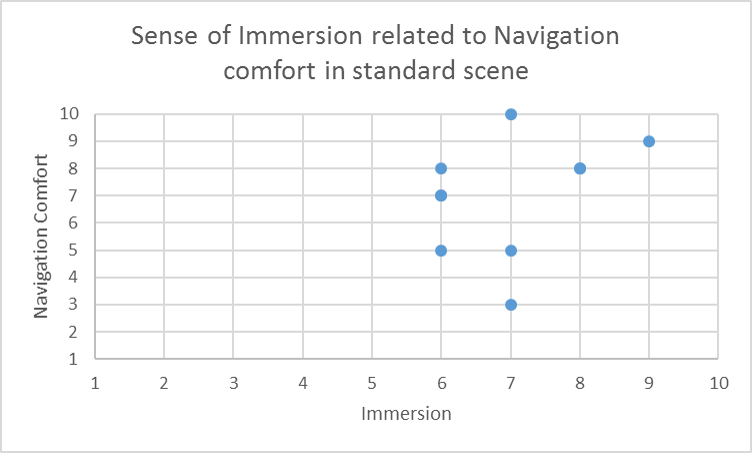
\includegraphics[width=1\textwidth]{Images/Standard_Relation}
					\centering
					\caption{Relation between sense of immersion and navigation comfort in standard geometry test scene, with trend line}
					\label{exp:fig:standard_relation}
				\end{figure}

		\subsection{Non-Euclidean Geometry}
		\label{exp:exp:ne}

			Similar to the standard Euclidean scene, after viewing the non-Euclidean scene participants were asked to answer questions relating to two main metrics, their sense of immersion, and comfort navigating the scene.

			\subsubsection{Immersion}

				As with the standard scene, participants immersion was rated on a scale of 1 - 10.
				For the results gathered for the non-Euclidean scene (\autoref{exp:fig:ne_immersion}), there was a mean value of $7$ which is the same as the standard scene (\autoref{exp:fig:compare_immersion_variation}), however for this scene there was a higher standard deviation, at $1.342$ (4 Significant Figures).

				Although there is a higher standard deviation in this scene compared to the standard Euclidean scene, the mean ($7$), and upper bounds ($9$) of the results are the same.
				If the outlier result of the non-Euclidean scene ($4$) is excluded from the result data, the mean value of the immersion rating for the scene increases to $7.\dot{3}$.

				\begin{figure}[h]
					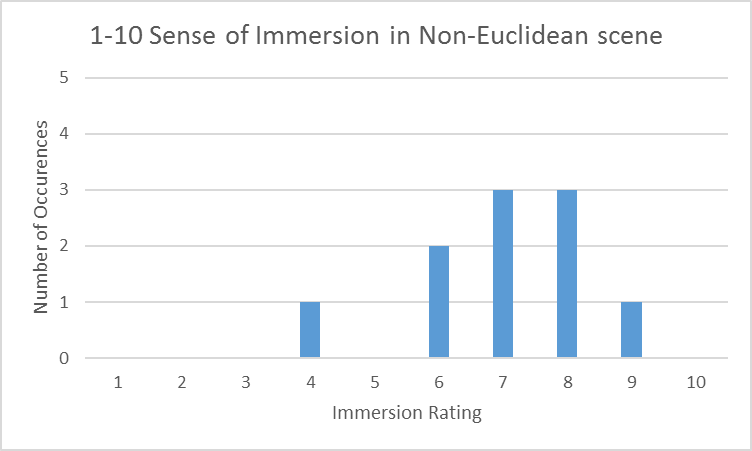
\includegraphics[width=1\textwidth]{Images/NE_Immersion}
					\centering
					\caption{Immersion rating in Non-Euclidean geometry test scene}
					\label{exp:fig:ne_immersion}
				\end{figure}

				$40\%$ of the comments regarding factors impacts in the sense of immersion within the scene mention the \enquote{puzzling} nature of the layout as a positive influence.
				Similar to the standard scene, a further $40\%$ also mention the head tracking making a positive impact on their sense of immersion.

				For this scene, $50\%$ of participants mentioned the movement input as a negative impact on their sense of immersion, $10\%$ more than in the standard scene.

			\subsubsection{Navigation Comfort}

				Navigation comfort for the non-Euclidean scene was also rated on a scale from 1 - 10.
				The gathered results (\autoref{exp:fig:ne_comfort}) for the non-Euclidean scene show a mean value of $6.2$ and a standard deviation of $1.6$.

				The mean value for this scene is lower than the standard Euclidean scene, however the standard deviation for the results is also lower.
				The lower standard deviation for this scene shows that, even though the mean value was lower, participants were more consistent in their comfort navigating within the scene.
				The consistency in the feedback for this scene could be due to participants having additional factors to focus on compared to the standard scene.

				\begin{figure}[h]
					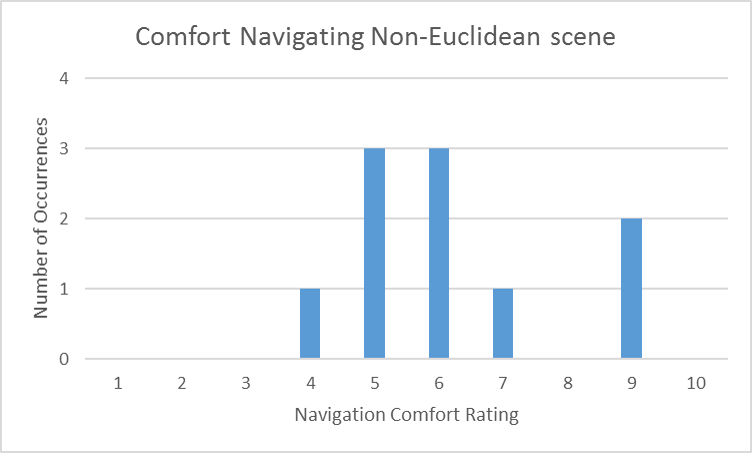
\includegraphics[width=1\textwidth]{Images/NE_Comfort}
					\centering
					\caption{Navigation Comfort rating in Non-Euclidean geometry test scene}
					\label{exp:fig:ne_comfort}
				\end{figure}

			\subsubsection{Correlation}

				As with the data gathered for the standard scene, the results for the immersion and navigation comfort in the non-Euclidean scene can be mapped on a scatter graph (\autoref{exp:fig:ne_relation}) to analyse any correlation between the data.

				Although there is still a slight positive trend between the two metrics for this scene, the magnitude of the trend line is significantly lower than in the standard Euclidean equivalent.
				For this scene, the trend line for immersion and navigation comfort fits on the line of $y = 0.3333x + 3.8667$.
				Because of how low the magnitude of the trend line is for this set of data, the positive correlation that is shown is not high enough for it to be valid evidence for actual correlation, with there being examples of participants who gave ratings in opposite extremes for either metric.

				\begin{figure}[h]
					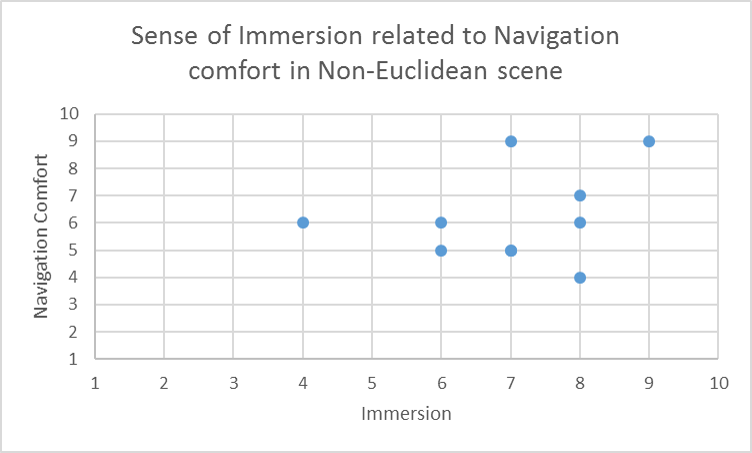
\includegraphics[width=1\textwidth]{Images/NE_Relation}
					\centering
					\caption{Relation between sense of immersion and navigation comfort in Non-Euclidean geometry test scene, with trend line}
					\label{exp:fig:ne_relation}
				\end{figure}

		\subsection{Experiment Comparisons}
		\label{exp:exp:comp}

			As well as analysing and comparing the individual scenes to each other, the order of viewing of the scenes has the potential of impacting the sense of immersion of the participant.
			In Experiment 1, participants viewed the standard Euclidean scene first, followed by the non-Euclidean scene.

			When directly comparing the immersion rating the participant gave in experiment 1 for each scene (\autoref{exp:fig:compare_immersion_exp1}), it can be seen that in $60\%$ of cases, participants found the non-Euclidean scene to be more immersive than the standard scene.
			As well as this, the remaining $40\%$ of participants had no change in their sense of immersion between the two scenes.
			This indicates that if a participant views a standard Euclidean environment prior to viewing a non-Euclidean environment, their sense of immersion will increase with the change.

			\begin{figure}[H]
				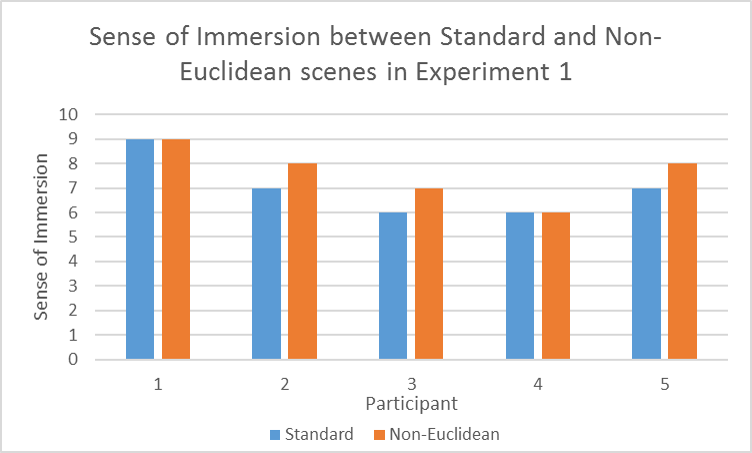
\includegraphics[width=1\textwidth]{Images/Compare_Immersion_Exp_1}
				\centering
				\caption{Comparison of participants sense of immersion in the two test scenes, from Experiment 1}
				\label{exp:fig:compare_immersion_exp1}
			\end{figure}

			In Experiment 2, participants viewed the non-Euclidean scene first, followed by the standard Euclidean scene.
			When the immersion ratings of the two scenes in Experiment 2 are directly compared (\autoref{exp:fig:compare_immersion_exp2}), there is a much more varied change in immersion between the two scenes compared to Experiment 1.

			By transitioning from non-Euclidean to Euclidean scenes, $20\%$ of participants felt the change decreased their sense of immersion.
			A further $40\%$ of participants found the change in Experiment 2 had no impact in their sense of immersion.
			The remaining $40\%$ of participants found that transitioning from non-Euclidean to Euclidean scenes positively influenced their sense of immersion.
			The varied results from Experiment 2 give no clear indication whether transitioning from a non-Euclidean scene to a Euclidean one effects a users sense of immersion either way.

			\begin{figure}[H]
				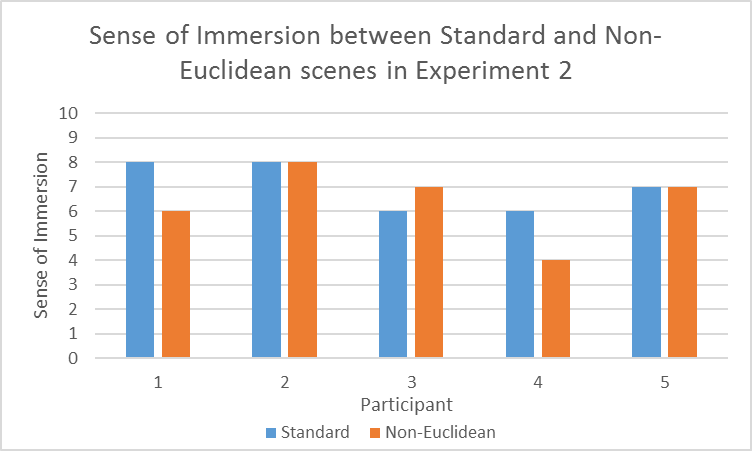
\includegraphics[width=1\textwidth]{Images/Compare_Immersion_Exp_2}
				\centering
				\caption{Comparison of participants sense of immersion in the two test scenes, from Experiment 2}
				\label{exp:fig:compare_immersion_exp2}
			\end{figure}

			% We kinda covered this in the previous subsections, so no need to directly reference it here
			\begin{figure}[H]
				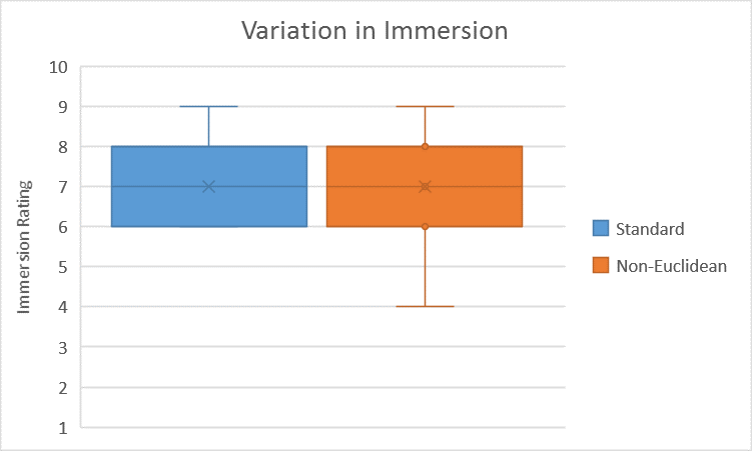
\includegraphics[width=1\textwidth]{Images/Compare_Immersion_Variation}
				\centering
				\caption{Mean values, and variation of Range for Immersion in the two test scenes}
				\label{exp:fig:compare_immersion_variation}
			\end{figure}

	\section[Summary]{Summary of Results}
	\label{exp:summary}

		The results of the experiments as a whole are interesting in the sense that they go against original expectations.
		The analysis of the results from Experiment 1 reveals that non-Euclidean geometry can have an effect on immersion in a virtual environment.
		The results show that if a participant transitions from Euclidean to non-Euclidean environments, their sense of immersion can be increased.
		This indicates that if non-Euclidean elements are added to a VR enabled virtual environment, it should be designed in a way that standard Euclidean geometry is experienced by the user beforehand.

		Results from Experiment 2 showed an absence of any significant difference in the effects of immersion when transitioning from a non-Euclidean to a Euclidean virtual environment.
		The lack of substantial differences in experiment 2 could be attributed to the relative simplicity of the standard scene when compared to the non-Euclidean one, with it appearing to a participant as the same scene, but with fewer things to do.
		This could be seen in a comment regarding a negative change in a participants immersion in the standard scene: \enquote{Not any different to the other one}.

		One consistency between the two experiments was the feedback that the input for movement within the scene could have been improved.
		Should further research be undertaken in this area, they might focus on the effects of control schemes or other impacts in navigation comfort.
